\chapter{Wprowadzenie}
\label{intro}
Niniejsza praca magisterska jest próbą rozwiązania problemu napotkanego w~mojej pracy zawodowej. Polegała ona na rozwijaniu rozproszonego systemu przeznaczonego do tworzenia i~wykonywania zautomatyzowanych testów. Można przyjąć, że system ten miał architekturę klient-serwer. Serwer uruchamiał na sobie testowany kod sparametryzowany danymi przesyłanymi przez klienta i następnie zwracał mu wyniki. Oba te elementy działały na platformie .NET pod Windowsem (oczywiście na różnych maszynach) i~komunikowały się przy pomocy Windows Communication Foundation (WCF, czyli web service'y Microsoftu). Całe to rozwiązanie miało już swoje lata (zaczęte jeszcze w .NET 2), było ciężkie w~utrzymaniu i~mało modularne. Tylko wspomnę, że wszystkie technologie i~techniki wymieniane w~tym i~następnych akapitach będą szerzej przybliżone w~dalszej części pracy.

Postawiono przede mną zadanie dodania do systemu możliwości uruchamiania testów na platformie Android. Wielki nacisk położono na kompatybilność wsteczną. Ponieważ w aplikacji klienta nie można było robić drastycznych zmian (takich jak przepisanie na inny język), nowy serwer na Androida (który miał zostać napisany w domyślnej dla tej platformy Javie) musiał tłumaczyć dane wejściowe i wyjściowe pomiędzy językami -- Javą a~C\#.  Właśnie to umożliwiają różne systemy zdalnego wywoływania kodu w środowiskach heterogenicznych, takie jak web service'y (jedną z~ich implementacji jest WCF). Niestety, Java na Androida -- a~ta różni się od standardowej -- nie ma żadnego odpowiednika serwera WCF. Trzeba go było stworzyć.

Mój system do RPC (\emph{Remote Procedure Call}, z~ang.\ zdalne wywoływanie metody) nie musiał się przejmować dużą częścią bolączek istniejących przemysłowych rozwiązań, takich jak kolejkowanie wiadomości, równoległa obsługa wielu klientów, czy bezpieczeństwo komunikacji. To dlatego, że model użycia był stosunkowo prosty -- na raz łączyły się tylko dwa węzły (klient i~serwer), a wszystkie dane (podróżujące w zaufanej wewnętrznej sieci) miały być łatwo podglądanie, aby wspierać debugowanie. Głównym problemem pozostało tłumaczenie danych. Udało mi się je zrealizować przez napisanie kodu w~Javie który serializował obiekty do XML w~taki sam sposób jak .NET (przy użyciu klasy DataContractSerializer) oraz potrafił deserializować XMLe od niego otrzymane. Ponieważ nie mogłem znaleźć żadnych zasad opisujących XMLe tworzone przez DataContractSerializer, sam musiałem je wydedukować poprzez analizę wyjścia dla różnych drzew obiektów, np. tablic, list, obiektów zawierających listy list itp. Takie podejście nie dawało, niestety, pewności, że program będzie działał poprawnie (a więc tak samo, jak .NET) dla wszystkich możliwych danych. Ale dla wszystkich z~jakimi został sprawdzony oraz dla tych które podawali użytkownicy (programiści piszący testy bazujące na naszym frameworku) działał, więc projekt został uznany za sukces.

Sukces ten jednak nie był bardzo satysfakcjonujący. Po pierwsze przez wspomnianą niepewność poprawności działania, po drugie przez to, że kod był słabej jakości. Co prawda działał poprawnie, ale był mało czytelny i zagmatwany. Po części to wina pośpiechu przy jego tworzeniu, po części tego, że kilka razy już po jego wprowadzeniu do użytku odkrywano nowe przypadki serializacji, które nieraz zmieniały założeniu już istniejące. Oczywiste stało się, że rozwiązanie trzeba było przepisać aby mogło żyć dalej i~stać się produktem, na którym można polegać. Co więcej tym razem trzeba było się dużo poważniej zastanowić nad miejscem mojej biblioteki w~ekosystemie systemów rozproszonych i nad uzasadnieniem jej stworzenia. Bo może jednak jest gdzieś na świecie coś, co spełniałoby nasz scenariusz użycia a~wcześniej zostało przeoczone. Albo przez ostatnie dwa lata, czyli od skończenia mojej pracy nad starym projektem, ktoś coś takiego stworzył.

Tak zostały wytyczone zgrubne cele niniejszej pracy magisterskiej: przeszukanie istniejącego oprogramowania w~celu wyłonienia kandydatów na gotowe rozwiązanie (bądź jego składniki), praktyczne porównanie możliwości istniejących bibliotek oraz w końcu, jeśli będzie taka potrzeba, stworzenie własnego produktu. Owocem mojej pracy powinno być coś, co przede wszystkim pozwoli zminimalizować nakład pracy programisty przy tworzeniu kanału komunikacyjnego między aplikacjami wykonanymi w~różnych technologiach, chociaż podstawowym celem jest łączenie Androida z~.NETem. To idzie w~parze z~wielkim atutem mojego programu -- dynamicznym (nie wymagającym specjalnych oznaczeń) polimorfizmem danych. Był już obecny nawet w~moim prototypie, a~nie jest cechą często spotykaną w~systemach RPC.

Aktualnie zakładam, że nowy system (owoc niniejszej pracy magisterskiej) będzie wykorzystywał mój format serializacji obiektów (danych) polegający na użyciu JSONa (lub jakiejś jego pochodnej) z~zapisywaniem dodatkowej informacji o~typie tychże obiektów dla wspomożenia polimorfizmu. Było już parę innych koncepcji (które będą przybliżone w~późniejszym rozdziale), a~dla jednej nawet powstał prosty prototyp, ale wszystkie zawierały jakąś poważną skazę. Ponieważ obecny pomysł zakłada, że zarówno biblioteka serwera (Android) jak i~klienta (.NET) będą potrafiły porozumiewać się w~obie strony tym samym językiem, nic nie stoi na przeszkodzie (poza czasem i~chęciami) aby powstały klienty i~serwery na inne platformy i~inne języki. Wnosi to chociażby tyle, że referencyjna implementacja obu części architektury może powstać w~Pythonie, który jest moim ulubionym językiem i~pozwala na szybkie przelewanie myśli na kod. W trakcie pracy przeprowadzę jeszcze sporo badań, co, mam nadzieję, dostarczy ostatecznego uzasadnienia aktualnej koncepcji systemu, ale może też zaowocować powstaniem nowej.

System który ostatecznie stworzę nie znajdzie, najprawdopodobniej, zastosowania w~przemysłowych projektach, ponieważ umyślnie będę pomijał niezbędne elementy dużych rozproszonych architektur -- bezpieczeństwo komunikacji, zrównoleglanie żądań itp. To, na czym głównie się skupiam, to pokazanie, że łączenie heterogenicznych aplikacji może być całkiem bezbolesne. W~trakcie pisania pracy będę brał pod uwagę jedynie współpracę dwóch programów na raz, ale małe sieci (do kilkunastu klientów na serwer) powinny również działać dobrze (co będę to sprawdzał). W przypadku, gdy mój projekt się powiedzie, to oczywiście będzie go można rozwijać dalej. Bycie otwartym i~publicznie dostępnym może tylko w~tym pomóc. Poza tym, jeśli znajdzie gdzieś rzeczywiste zastosowanie (co mnie by bardzo cieszyło, a~mu dałoby szansę na ``życie''), to najpewniej właśnie w~innych projektach z~domeny Open Source.

%Wydaje mi się, że niniejsza praca jest trudniejsza w~realizacji niż większość innych na naszym wydziale. Rzucony na otwartą wodę szerokiej dziedziny musiałem sobie radzić sam. Z~wytyczonym z~grubsza celem sam musiałem go dookreślić (aby w~ogóle powstał temat) i~wyszukać możliwe rozwiązania. Podczas gdy wiele prac polega na sprawdzeniu lub zrealizowaniu jednego pomysłu, ja musiałem najpierw stworzyć sam pomysł -- i~to nie jeden. Mimo, że mój ostateczny produkt nie powinien być bardzo skomplikowany (taką mam nadzieję), to droga, którą musiałem pokonać 
%wysiłek umysłowy potrzebny do odnalezienia się w~tym świecie i zaproponowaniu czegoś, czego jeszcze nie ma jest znaczny. Droga potrzebna do odnalezienia tego rozwiązania jest męcząca -- ją przedstawię. Cały czas się zastanawiam, czy ma to sens.

%Nie było tam za bardzo zarządzania połączeniami i innych cech dojrzałego systemu - tylko prosta map obietków i przesyłanie zserializowanych poleceń. Dlatego postanowiłem, że dobrze zrobić nowy system. Skoro i tak nie było to zgodne ze standardnem (własne łączenie, przesyłanie z serializowanych rzeczy), to nie jest dużym problemem wymienienie kawałka po stronie .NET (serializatora) i zrobienie tego tak, żeby było też ``wygodnie'' po stronie Javy. Czyli po prostu mieć kod po obu stronach, który wygląda (choć w innym języku) i zachowuje się tak samo. Poza tym brakuje takich rozwiązań, których można użyć we własnym projekcie bez używania jakiś standardowych i ciężkich rozwiązań. Poza tym, te rozwiązania i tak nie są zgodne i wspierają różne części standardu \emph{(Jakieś źródło)}.

\section{Cele pracy}
W tym miejscu zdefiniowane i uzasadnione zostaną cele niniejszej pracy.

%Każdy punkt powinien mieć dwie podsekcje - co? (wyjaśnia co dokładnie będzie zrobione) i dlaczego? (moje pobódki, co mi i innym to da). Jak? Po co? dla każdego celu zostanie odpowiedziane już w pracy.

\subsection{Przybliżenie tematyki}
Aby dało się zrozumieć pobudki, wywody oraz produkty tej pracy należy zaznajomić się z~tematyką zdalnego wywoływania kodu oraz charakterystyką docelowych platform. Zrobienie tego w~stopniu wystarczającym powinien umożliwić rozdział \ref{intro}.

\subsection{Porównanie istniejącego oprogramowania}
Przybliżone i~porównane zostaną co bardziej interesujące (dla mojego zastosowania) istniejące biblioteki oraz frameworki z~dziedziny RPC i~serializacji. Będzie to obszerna i~bardzo ważna część tej pracy.

Tylko przez takie badania można stwierdzić, że mój produkt znajdzie dla siebie jakąś niszę, a~zatem tworzenie go nie będzie pozbawione praktycznego sensu.

Technologie będą rozpatrywane w kategoriach:
\begin{itemize}
	\item obecności pożądanych przeze mnie cech (wymienianych w \ref{lib_requirements}),
	\item spełniania obietnic, co do swoich możliwości,
	\item zdolności współpracy z~innymi technologiami.
\end{itemize}

Po tej analizie stwierdzę na których rozwiązaniach mogę się wzorować lub wykorzystać jako elementy swojego.

\subsection{Stworzenie wieloplatformowej biblioteki}
\label{lib_requirements}
Oprogramowanie które stworzę będzie miało postać kilku (dwóch lub więcej) bibliotek na różne systemy. Każda z~nich będzie miała analogiczny interfejs i~taką samą funkcjonalność. Poniżej wyliczone są cechy, których obecność ma definiować moje rozwiązanie.

\begin{description}
\itemtitle{Wywoływanie kodu na Androidzie z~poziomu C\#}
Cel główny, w~końcu to jest mój problem wyjściowy. Moje dzieło ma pozwolić na wywoływanie metod (i~otrzymanie od nich wartości zwrotnych) napisanych w~języku Java pod Androidem przez program napisany w C\#. Można powiedzieć, że jest to zarządzanie Androidem z Windowsa (bo C\# działa na .NET, a ten z kolei domyślnie działa na Windowsie).

\itemtitle{Polimorfizm zdalnych metod}
Zdalne metody powinny być polimorficzne. To znaczy, że każdy z~ich argumentów (jeśli jest to metoda przyjmująca argumenty) nie jest ograniczony do przynależności do jednego typu\cite{polymorphism}. Będzie to osiągnięte na dwa sposoby. Pierwszy -- przeciążanie metod (polimorfizm ad-hoc), polega na tym, że może istnieć zbiór różnych metod o~tej samej nazwie, pod warunkiem, że przyjmują różne zestawy argumentów. Drugi -- to nadanie argumentom cechy nazywanej z~angielskiego \emph{inclusion polymorphism}. Można by to przetłumaczyć jako polimorfizm zawierania. Znaczy to tyle, że jeden typ posiada te same metody i~pola co inny typ (zawiera go); najczęściej posiada też właściwe dla siebie cechy (metody i~pola). W~językach obiektowych zazwyczaj taki polimorfizm realizowany jest przez dziedziczenie -- jeden typ dziedziczy po drugim, w ten sposób przejmując jego cechy. Dzięki temu typ dziedziczący może być traktowany tak samo, jak typ dziedziczony. Podsumowując, pod każdy argument zdalnej metody można podstawić zarówno wartość typu określonego przez nią oczekiwanego, jak i dowolnego typu dziedziczącego po nim.

%Nie zapewnie polimorfizmu parametrycznego, czyli szblonów.

\itemtitle{Swoboda rozszerzania kodu}
Raz napisany kod zawierający moje zdalne metody powinien być rozszerzalny bez potrzeby jego zmiany \cite[str.~105]{designpatterns}. Jest to jedna z~podstaw obiektowego podejścia do programowania. Umożliwia jej działanie, między innymi, polimorfizm. Dla przykładu -- raz stworzonej zdalnej metodzie mogę przekazać argument nowego typu, który dziedziczy po spodziewanym. Przypuśćmy dalej, że metoda uruchamia jakąś metodę parametru, który otrzyma, a~ta metoda została rozszerzona w podtypie. Tym samym stara metoda zaowocuje uruchomieniem nowego kodu, a~ani jej, ani oryginalnego typu parametru nie trzeba było zmieniać.

\itemtitle{Prostota użycia}
Moja biblioteka powinna pozwalać na szybkie tworzenie zdalnych metod w~prosty sposób. Jej instalacja ma być oczywista, API przejrzyste. Jeśli wymagana będzie konfiguracja to powinna być krótka i~zrozumiała. Jeśli trzeba będzie tworzyć opisy umożliwiające tłumaczenie obiektów danych (przedstawicieli klasy bez metod) z~jednego języka na odpowiadające obiekty w~drugim języku drugi, to powinny być one generowane automatycznie przy minimalnej ilości parametrów. Moje oprogramowanie może także mieć możliwość wygenerowania kodu klasy (danych) w~jednym języku na bazie kodu klasy napisanej w~drugim. Ogólnie powinno zdejmować z~programisty możliwie dużo trosk (zadań), które nie wymagają interwencji istoty obdarzonej zdolnością abstrakcyjnego myślenia i~mogą być rozwiązane przez automat.

\itemtitle{Wsparcie wielu środowisk}
Cel drugorzędny, do którego nie będę przywiązywał wielkiej wagi. Ale jeśli uda się umożliwić łączenie tak różnych środowisk jak Android (który jest platformą mobilną, a~więc ograniczoną) i~.NET, to może nie będzie wielkim problemem wsparcie kolejnych platform. Może połączenie tych środowisk będzie rozwiązywało na tyle uniwersalne problemy, że dodanie klienta/serwera dla, chociażby, Pythona, Windows Phone lub innych platform (w~tym osadzonych) będzie procesem, który można wykonać bez większej refleksji. 
\end{description}

Istnieją zagadnienia ważne dla aplikacji rozproszonych, które będą przeze mnie pomijane, aby nie przesłaniać najważniejszych (według mnie) kwestii. Moja praca nic do nich nie wniesie, więc nie ma sensu się nimi zajmować. Są to, między innymi (bo nie sposób wymienić wszystkiego, co \emph{nie} wchodzi w~obszar zainteresowań):

\begin{description}
\itemtitle{Bezpieczeństwo komunikacji}
Krytyczny czynnik dla aplikacji rozproszonych \cite[str.~21]{webservices}. Polega na zapewnienie poufności, uwierzytelniania (i~autoryzacji) i~spójności/nienaruszalności. Spójność można rozważać zarówno w~kontekscie zapewnienia poprawności danych przesyłanych przez sieć \cite{dataintegrity}, jak i~zagwarantowaniu, że odbiorca będzie mógł zidentyfikować i~odrzucić wiadomość, która została przez kogoś celowo zmodyfikowana po wyjściu od nadawcy \cite{datasignature}. Nie będę starał się ich zapewnić, ale jako osoba praktykująca nie mogę całkiem o~nich zapomnieć. Dlatego jeśli nie będzie mnie to spowalniać, będę zostawiał miejsca, w~których będzie można zapewnić bezpieczeństwo przez dodanie lub wymianę modułu aplikacji. Na przykład przez zastąpienie zwykłych połączeń TCP (które i~tak zamierzam traktować abstrakcyjnie) połączeniami TLS (które tak naprawdę są nakładką na TCP \cite[str.~47]{tls}).

\itemtitle{Wydajność}
Jest niezmiernie ważna dla wszystkich serwerów, ponieważ muszą obsługiwać wielu klientów na raz. Jednak moja aplikacja nie musi być tak wydajna, nie muszę przejmować się ``odmową usługi'' \cite{dos}(z~ang. DoS, \emph{Denial of Service}) przez serwer. Z~doświadczenia wiem, że program typu tworzonego przeze mnie, rozmawiający na raz z~kilkoma--kilkunastoma klientami nie powinien mieć problemów z~nadążeniem, jeśli nie będzie w~nim rażących błędów. Taka ilość połączeń póki co całkowicie mnie zadowala. Tym bardziej, że mój system wyjściowo miał działać przy połączeniu ``1 do 1'', jako most między dwiema aplikacjami. Zajmuję w~tym przypadku podobną postawę wobec wydajności, co wobec bezpieczeństwa -- mimo ich pomijania dalej jestem świadom problemów z~nią związanych i~jeśli nie będzie to w~żaden sposób problematyczne będę zapewniał względną (względem czytelności) optymalność kodu.
\end{description}

%Ale ponieważ nie sposób choć trochę o~nich nie myśleć przy projektowaniu tego typu systemu, b to jeśli będzie to sprawiało minimalny problem, będę starał się o nie zadbać
%dążył do jak najwyższej ich wartości, albo zostawiał miejsce na ich zapewnienie w przyszłości.

%\section{Używany język (TODO)}
%W~pierwszym zdaniu tej pracy najprawdopodobniej rzuciła się Tobie, czytelniku, od razu w oczy nieformalna konstrukcja. Mogła nawet w~nie razić. Mimo, że może się ona wydawać nieadekwatna, to przenosi nie mniej informacji niż bezosobowe stwierdzenie ``w~pracy zawodowej autora'', a~jest dla mnie -- tegoż właśnie autora -- przyjemniejsza w~użyciu, a~zatem lepsza. Więcej o~tym później.
%
%Napisać o tym, że język w mojej pracy może nie być do końca formalny. Mogę wtedy przekazywać informacje tak samo dobrze albo nawet lepiej (bo mogę być bardziej obrazowy, a nie muszę być od razu nieprecyzyjny) a zarówno pisanie jak i czytanie pracy będzie przyjemniejsze. Nauka powinna być frajdą. Coś przytoczyć może z tego headfirsta albo ich źródeł? W anglojęzycznej literaturze, która jest w sumie światowym standardem naukowym (jakiś cytat znaleźć) często tworzą jakieś nieformalne konstrukcje (sandwiche, cargo cult programming). Cytat z Head firsta o tym, że jak jest rozmowa to się lepiej czyta i pamięta. A zakładam, że ktoś poza mną przynajmniej raz będzie to czytał i chociaż jego zadanie będzie przyjemniejsze. Moje na pewno. Niby praca dyplomowa ma być napisana jasno i konkretnie (\url{http://www.slideshare.net/jszypryt/prace-dyplomowe-i-ich-cele-rodzaje-i}), a takie bezosobowe ściemnianie jest oczywistym tego przeciwieństwem. Bo przecież napisanie, że jakiś program ``zrobiono'' albo, że ``powstał'' ukrywa prawdę, że to właśnie JA zrobiłem. Za często trzeba się zastanawiać jak coś trafnie sformułować, żeby nie brzmiało nazbyt potocznie. Zdecydowałem się odrzucić takie problemy. Uznaję, że jeśli tekst przekazuje informacje precyzyjnie i zrozumiale dla osoby posługującej się współczesnym językiem polskim to jest to tekst poprawny.
%
%\emph{Mam jakies rzeczy w downloadsach.} \\
%\url{http://galaxy.agh.edu.pl/~wkowalsk/dydaktyka/skrypt.pdf}\\
%\url{http://chomikuj.pl/miechu17/Ksi*c4*85*c5*bcki/Uwagi+o+pisaniu+i+redagowaniu+prac+dyplomowych+na+studiach+technicznych+-+E.+Opoka,3372705642.pdf}\\
%\url{http://dyplom.best4u.pl/zasady-pisania-prac-dyplomowych}\\
%\url{http://zwa.univ.szczecin.pl/wp-content/uploads/2013/04/zasady-pisania-prac-dyplomowych_2012_2013.pdf}\\
%\url{http://www.slideshare.net/jszypryt/prace-dyplomowe-i-ich-cele-rodzaje-i}\\
%\url{http://www.ithg.wsg.byd.pl/userfiles/files/II%20Uwagi%20dotycz%C4%85ce%20pisania%20prac%20seminaryjnych(1).pdf}\\
%\url{http://dydaktyka.polsl.pl/kwmimkm/jak_pisac.pdf}\\
%\url{http://www.maraton.home.pl/por_aut.htm}\\
%
%Książki O'Reilly i Head First na przykłady. W ``On Understanding Types, Data Abstraction and Polymorphism.pdf'' nawet jest ``set of clothes'' i ``naked'' representation.

\section{Docelowe platformy}
Tutaj zostaną opisane platformy technologiczne, na których będzie działać moja biblioteka.

\subsection{Android}
%moze dodac odniesienie do kilku rozdzialow learningandroid od razu przy tym rozdziale, a nie gdzies w tekscie? tak się robi?

\subsubsection{Omówienie}
Android jest kompletną, otwartą (open-source) platformą dla urządzeń mobilnych opartą o~Linux\cite{learningandroid}. Został stworzony przez organizację Open Handset Alliance. Organizacja skupia wielu operatorów komórkowych, producentów elektroniki, telefonów i~oprogramowania oraz firmy komercjalizacyjne \cite{oha}. Pomysłodawcą uformowania oraz liderem tej organizacji jest firma Google. Jej misją jest przyspieszenie innowacji na platformach mobilnych oraz dostarczenie konsumentom pełniejszego, tańszego i~ogólnie lepszego doznania z~korzystania z~telefonu. Wszystko to za sprawą Androida, który dodatkowo jest całkowicie otwarty.

Krótka historia systemu, która powinna rzucić na niego trochę światła:
\begin{itemize}
	\item W 2005 roku Google kupuje Android, Inc. -- świat oczekuje pojawienia się telefonu Googla (``gPhone'').
	\item Długa cisza.
	\item 2007, ogłoszenie zawiązania Open Handset Alliance i~pojawienie się Androida.
	\item 2008, wypuszczenie Android SDK 1.0 (o~tym niżej); krótko po tym wypuszczenie pierwszego telefony z Androidem -- HTC G1.
	\item 2009, telefony z Androidem coraz powszechniejsze (ponad 20 modeli), współistnieje wiele wersji systemu: Cupcake(1.5), Donut(1.6), Eclair(2.0, 2.1).
	\item maj 2010, Android jest drugim (po Blackberry) pod względem popularności systemem dla smartfonów; wypuszczenie Froyo(2.2) i~ponad 60 modeli telefonów go posiadających.
	\item grudzień 2010, wielkie zmiany (poprawki) w~interfejsie użytkownika wprowadzone w~wersji Gingerbread(2.3).
	\item luty 2011, wydanie Honeycomb(3.0)\cite{androidhistory}. Został wydany tylko na tablety, co przeczyło założeniu systemu uniwersalnego dla różnych urządzeń. Jego źródła nie zostały otwarte tym samym łamiąc obietnice całkowitej otwartości.
	\item październik 2011, Ice Cream Sandwich(4.0) wraca do ideałów będąc otwartym systemem zarówno na telefony, jak i~tablety (i~dowolne inne urzdzenia)
	\item 2014, zapowiedź Androida L, który ma znacznie zwiększyć wydajność (dzięki nowemu podejściu do kompilacji aplikacji\cite{androidart}), poprawić interfejs użytkownika i~wspierać aplikacje 64-bitowe\cite{androidlogolnie}.
\end{itemize}

Jako że Android jest przeznaczony dla urządzeń mobilnych, jego twórcy musieli wziąć pod uwagę ograniczenia, które miały być względnie niezmienne w~przewidywalnym czasie.
To, że telefony są zasilane z~baterii (których pojemność bardzo się nie zmienia) oraz nieduży rozmiar, ograniczają moc procesora i~możliwą pamięć. Mimo tego, użytkownik powinien być zadowolony z~szybkości urządzenia, tak samo jak w~przypadku zasobożernych komputerów osobistych.
Rozwiązanie tego problemu wymaga dużej pomysłowości i~musi owocować pewnymi kosztami.

Ten system zrewolucjonizował rynek mobilny (i~nie tylko). Pierwszy raz otwarta platforma rozdziela sprzęt od oprogramowania na nim działającego. Ponieważ jej rdzeń jest przenośny i~nie ma założeń co do sprzętu, pozwala dużo większej niż do tej pory liczbie urządzeń na uruchamianie tych samych aplikacji i~tworzy bogatsze środowisko, zarówno dla programistów, jak i~konsumentów. Nie ogranicza się tylko do telefonów, tabletów, i~laptopów, ale zaczyna występować nawet w~telewizorach, samochodach i, zdaje się, wszystkich innych urządzeniach w~których można osadzić mikrokomputer\footnote{Np. w~lodówkach \url{http://venturebeat.com/2013/01/11/samsung-smart-fridge-it-runs-android-apps-like-evernote-video-demo/}}.

Użytkownicy zauważą, że działa w~pełni od razu po zakupie urządzenia, bez potrzeby skomplikowanej konfiguracji. Mogą też go mocno zmodyfikować dopasowując go do swoich potrzeb.
Programistom dostarcza kompletny zbiór narzędzi -- Android SDK (Software Development Kit) -- potrzebnych do łatwego i~szybkiego tworzenia aplikacji. Nie ma nawet potrzeby posiadania fizycznego urządzenia, ponieważ Android SDK zawiera emulator.
Producenci mogą go widzieć jako kompleksowe rozwiązanie na oprogramowanie swoich urządzeń. Jedyne, czego brakuje Androidowi do nadania życia urządzeniu to warstwa sterowników bezpośrednio związana ze sprzętem.

Każdy element systemu jest objęty licencjami przyjaznymi dla firm komercyjnych (Apache, MIT), aby mógł być swobodnie rozszerzany i~używać dla różnorakich celów.
Jeśli jakiś producent sobie tego życzy, to może nie ujawniać części, które sam dodał. Ale poza tym, reszta systemu jest otwarta i~każdy może ją ściągnąć\footnote{Instrukcje można znaleźć tu: \url{https://source.android.com/source/building.html}} i~przejrzeć, albo nawet zmodyfikować.
Niektóre z~otwartych bibliotek, które były wcielone do systemu, zostały nawet przepisane specjalnie po to, aby objąć nadać im takie licencje.

\subsubsection{Programowanie}
System jest niejako nadbudówką na Linuxa, dojrzałą chlubę ruchu open-source. Android dziedziczy jego dobre (i~pozostałe) cechy jak bezpieczeństwo, przenośność, czy zespół solidnych (ang. \emph{robust}) zasad zarządzania zasobami, a~także bogaty asortyment rozwijanych latami narzędzi.

Ma strukturę warstwową. Każda warstwa ma własną charakterystykę i~przeznaczenie. Nie są one, jednak, od siebie idealnie rozdzielone i~częściowo na siebie zachodzą.

Android jest platformą kompletną (ang. \emph{comprehensive platform}), co znaczy, że zawiera pełny stos oprogramowania dla urządzenia mobilnego. Stos ten zawiera wszystko od niskopoziomowych modułów jądra Linuxa, przez biblioteki natywne, platformę aplikacji (ang. \emph{framework}) po same aplikacje (widoczny na rysunku \ref{fig:android_architecture}).

\begin{figure}
	\centering
		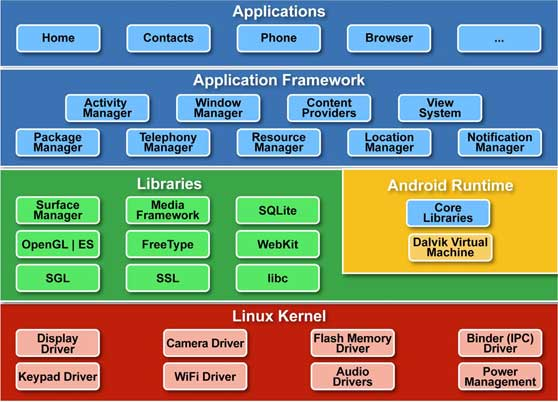
\includegraphics[scale=0.7]{img/android_architecture.jpg}
	\caption{Stos Androida, źródło: \cite{androidstack}}
	\label{fig:android_architecture}	
\end{figure}

Jeśli chodzi o~kod natywny(C/C++), to można na niego programować mniej więcej tak, jak na ``standardowego'' Linuxa. Ma podobny zestaw bibliotek. Część została włączona do systemu bez zmian. Ważnym wyjątkiem jest Bionic -- alternatywna implementacja biblioteki standardowej C (\emph{libc}). Google zdecydował się na jej przepisanie aby zoptymalizować ją pod urządzenia z~ograniczonymi zasobami oraz żeby uniknąć problemów licencyjnych związanych z~``infekcją'' przez licencję GPL (którą objęta jest \emph{libc}).

Trzeba powiedzieć, że pisanie programów w~C nie jest zalecanym sposobem pisania aplikacji na Androida. Podstawowym językiem jest Java. API dla tego języka dostarczane przez Google pozwala na budowanie programów, które klasyfikowane są jako aplikacje Androidowe. Te aplikacje przyjmuję postać paczek APK (Application Package). Mogą one być łatwo instalowane i~wykorzystywane przez zwykłych użytkowników.

Java, w~przeciwieństwie do np.~C nie jest kompilowana do kodu maszynowego, który może być wykonany przez procesor. Zamiast tego jest kompilowana do kodu bajtowego Javy (\emph{Java bytecode}), który abstrahuje od właściwości (takich jak architektura procesora) komputera, na którym ma być wykonany \cite{jvm}. Za przełożenie wykonywanego kodu na prawdziwe instrukcje procesora, zwane JIT -- z~ang. \emph{just-in-time compilation}, a~więc kompilacja w~samą porę, jest odpowiedzialna maszyna wirtualna Javy (ang.: \emph{Java Virtual Machine (JVM)}). JVM posiada różne wersje (wszystkie zgodne z~jedną specyfikacją) dopasowane do środowisk, w~których mają działać. Inna będzie potrzebna na Linuxa, inna na Windowsa. Ale każda z~nich powinna być w~stanie wykonać z~takim samym efektem taki sam kod Javy. Zatem teoretycznie można napisać jeden program, który bez żadnych modyfikacji będzie działał na całkowicie odmiennych systemach operacyjnych.

Na potrzeby Androida stworzona została nowa, otwarta JVM o~nazwie Dalvik. Dalvik jest zoptymalizowany na urządzenia mobilne. Faktycznie operuje na innym niż standardowy kod bajtowy, ale kod dla Dalvika uzyskuje się przez dodatkową kompilację (optymalizację) zwykłego kodu bajtowego (zilustrowane na rysunku \ref{fig:dalvik-compilation}). Teoretycznie, każdy język kompilowany do kodu bajtowego Javy (a~jest ich kilka, np. Scala) powinien móc być wykonany na Dalviku.
Poza tym, nowa maszyna wirtualna była potrzebna aby uniezależnić się od właściciela Javy (kiedyś Sun, obecnie Oracle). Narzędzia do język (jak kompilatory) i~standardowe odmiany JVM są darmowe, ale należą do Oracle, a~ich kod nie jest otwarty. Istnieją też, co prawda, alternatywne otwarte implementacje JVM, jak ta dostarczana z OpenJDK.

\begin{figure}
	\centering
		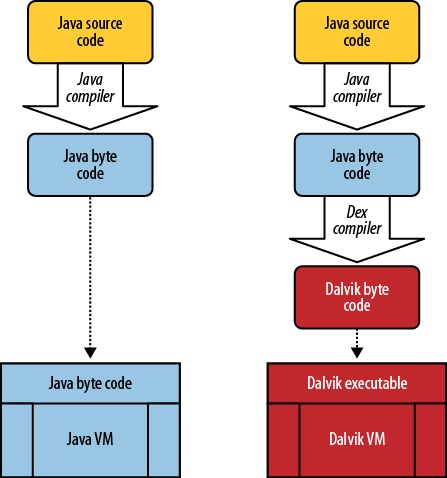
\includegraphics[scale=0.75]{img/dalvik-compilation.jpg}
	\caption{Porównanie standardowej kompilacji Javy z~kompilacją dla Dalvika. Źródło: \cite{learningandroid}}
	\label{fig:dalvik-compilation}
\end{figure}

Aktualnie istnieje już następca Dalvika -- Android Runtime (ART). Wprowadzono go jako alternatywną maszynę wirtualną w~ostatnim Androidzie (4.4)\cite{androidart}. W~kolejnej wersji systemu -- Androidzie L -- będzie już domyślny\cite{androidlpreview}. Jego głównym celem jest przyspieszenie wykonywania aplikacji. Osiąga to przez usprawnione odśmiecanie pamięcie (ang. \emph{garbage collection}) oraz przez wprowadzenie techniki określanej jako \emph{ahead-of-time compilation} (AOT), czyli kompilacja przed czasem (kontrast dla JIT). AOT polega na tym, że w~trakcie instalacji aplikacja (skompilowana do kodu Dalvika) jest kompilowana jeszcze raz, już na kod maszynowy dopasowany do urządzenia, na którym odbywa się instalacja. Przez to zużywane jest dodatkowe miejsce, ale aplikacja może się wykonywać szybciej, ponieważ jej kod nie musi być interpretowany przez JVM.

Java która jest dostępna na Androidzie niestety nie ma pełnego zbioru standardowych bibliotek (z~Javy SE). Między innymi, brakuje wielu części pakietu \emph{javax}. Niektóre rzeczy, za które były one odpowiedzialne to świadczenie i~konsumowanie usług internetowych (bycie serwerem lub klientem dla web service'ów), czy interfejsy użytkownika (Swing, AWT). W~zamian zostały dodane pakiety ułatwiające pisanie aplikacji pod Androida. Umożliwiają one komunikację aplikacji między sobą i~z~systemem, składowanie danych, dostęp do sensorów i~funkcji telefonu oraz wiele inne przydatnych działań\cite{androidpackage}. Wśród nich są też biblioteki odpowiedzialne za GUI Androida. Dzięki nim wszystkim ekosystem (programów) jest dość jednorodny i~ustandaryzowany.

Od jakiegoś czasu Java nie jest jedynym językiem, w którym można pisać aplikacje. Co prawda już kiedyś można dodać do APK bibliotekę C/C++ (pisaną przy użyciu NDK -- Native Development Kit\cite{androidndk}) i~wołać ją z~Javy, ale zawsze potrzebny był Javowy szkielet. Teraz można oznaczyć, że APK korzysta z~\emph{NativeActivity}\cite{androidnativeactivity}, co pozwala całość zaimplementować natywnie. 

Warto też powiedzieć, że każda aplikacja instalowana z~APK jest identyfikowana jako odrębny Unixowy użytkownik\cite{androidpermissions}. Dzięki temu można precyzyjnie zarządzać tym, do czego dana aplikacja ma dostęp, co zwiększa ogólne bezpieczeństwo systemu. W~systemach instalowanych na telefonach standardowo jest blokowane konto administratora systemu (\emph{root}). Użytkownik może je odblokować przez zabieg zwany rootowaniem.

Android nie ogranicza się do uruchamiania jedynie kodu napisanego w~C, C++ lub Javie (uznajmy je za języki ``standardowe''). Istnieje aplikacja działająca jako interpreter innych języków -- SL4A\cite{androidsl4a} -- która pozwala wykonywać skrypty napisane w~kilku językach, m.in.\ Python, Perl, Lua, JavaScript.\footnote{Inną aplikacją tego typu jest QPython (\url{http://qpython.com/}), która zawiera SL4A.}
Są też kompilatory tworzące kod bajtowy Dalvika z~języków inne niż standardowe (dla Androida). Tu przykładem jest Xamarin \footnote{\url{http://xamarin.com/}}, rozwiązanie umożliwiające pisanie w~C\# aplikacji na kilka platform, w~tym Androida.
Jednak zarówno SL4A i~Xamarin nie dają dostępu do wszystkich standardowych bibliotek. Jest tak dlatego, że użycie API Androida w~kodzie niestandardowego języka wymaga zmapowania do niego tychże API, co jest czasochłonne i~trudne do wykonania w~całości przez kogoś innego niż Google. Ponadto, niestandardowy dla Androida język, taki jak C\#, może mieć struktury, które nie dadzą się przetłumaczyć na kod bajtowy Javy. Tym samym nie będzie można go wykorzystać w~pełni. Odmiennym przypadkiem jest język Scala. Dzięki zgodności na poziomie kodu bajtowego (bo tak samo jak Java jest do niego kompilowana) Scala może być użyta do stworzenia kompletnego APK mającego dostęp do wszystkich bibliotek.

%Może wypunktowana lista ze wspieranymi językami? Tu macie języki i jak mocno i przez co są wspierane (może tabelka? nazwa | czy można całą aplikację w tym zrobić | jakiś opis, przez co dostarczane, uwagi). Dalej co ważniejsze opisane. Oczywiście jest więcej.
%\url{http://www.dobreprogramy.pl/Google-testuje-nastepce-Dalvika-z-ARTem-Android-bedzie-dwukrotnie-szybszy,News,49129.html}
%\url{http://stackoverflow.com/questions/3316801/which-programming-languages-can-be-used-to-develop-in-android}
%\url{http://en.wikipedia.org/wiki/Android_software_development}
%https://github.com/jberkel/android-plugin
%https://github.com/jberkel/android-plugin/wiki/getting-started
%http://www.scala-sbt.org/release/tutorial/index.html

\subsection{.NET}
.NET to technologia stworzona przez Microsoft, wspomagająca tworzenie i~uruchamianie aplikacji (w~tym usług sieciowych), głównie dla systemu Microsoft Windows\cite{dotnetoverview}. Jego główne cele:
\begin{itemize}
	\item Zapewnić jednorodne środowisko do programowania obiektowego, zarówno dla kodu lokalnego wykonywanych lokalnie, kodu rozproszonego wykonywanego lokalnie, czy wykonywanego w~całości zdalnie.
	\item Minimalizacja ilości zależności aplikacji oraz konfliktów wersji.
	\item Krzewienie bezpiecznego wykonywania kodu, także od nieznanych lub częściowo zaufanych źródeł.
	\item Zlikwidowanie problemów wydajnościowych skryptów oraz kodów interpretowanych (nienatywnych).
	\item Zapewnić jednolity styl programowania na różnych platformach, np. przy aplikacjach okienkowych Windows i~aplikacjach internetowych.
	\item Oparcie całej komunikacji o~obowiązujące standardy, aby kod napisany pod .NETem mógł się integrować z~dowolnym innym kodem.
\end{itemize}

Cała platforma składa się z~dwóch elementów -- środowiska uruchomieniowego języka wspólnego (ang. \emph{common language runtime}) oraz biblioteki klas. Środowisko uruchomieniowe jest podstawą całej platformy. Przypomina maszynę wirtualną Javy (można je też samo nazywać maszyną wirtualną), będąc agentem, który zarządza kodem w~trakcie jego wykonywania, dostarczając przy okazji kluczową funkcjonalność jak zarządzanie pamięcią, wątkami, zdalne wywoływanie, wymuszanie bezpieczeństwa typów (ang. \emph{type safety}) i~innych form poprawności kodu zapewniających bezpieczeństwo i~solidność programów.

Kod wykonujący się w~środowisku uruchomieniowym zwany jest kodem zarządzanym (ang. \emph{managed code}). Pozostały kod, jak natywny, nazywany jest kodem niezarządanym (ang. \emph{unmanaged code}). Kod zarządzany jest kompilowany do Wspólnego Języka Pośredniego\cite{cil} (ang. \emph{Common Intermediate Language, CIL}), który można porównać do kodu bajtowego Javy, choć jest bardziej czytelny dla człowieka. Podobnie cechuje go niezależność od sprzętu i~systemu operacyjnego.

Biblioteka klas jest obszernym zbiorem gotowych typów zgodnych z~zasadami programowania obiektowego, mogących służyć za gotowe komponenty różnych aplikacji. Są tam elementy do tworzenia aplikacji graficznych (GUI), internetowych (ASP.NET, Web Forms), kryptograficznych, czy całych usług internetowych (\emph{web services}) i~wiele innych.

Środowisko uruchomieniowe .NET może być osadzane w~aplikacji niezarządzanej w~celu ładowania kodu zarządzanego, tym samym tworząc środowisko mogące korzystać z~cech zarówno niezarządzanego jak i~zarządzanego kodu. Platforma dostarcza kilku takich ``gospodarzy'' (\emph{hosts}) dla środowiska uruchomieniowego, wspomaga też ich tworzenie przez osoby trzecie.
Warto zaznaczyć, że Java również może być w~podobny sposób osadzana.
Przykładami gospodarzy dla środowiska .NET mogą być ASP.NET (``framework'' do budowy aplikacji internetowych) lub Internet Explorer.

Na rysunku \ref{fig:dotnet-ecosystem} przedstawione są zależności środowiska uruchomieniowego języka wspólnego (\emph{runtime}), biblioteki klas, systemu operacyjnego i~aplikacji użytkownika. Widać też gdzie działa kod zarządzany (\emph{managed code}) względem niezarządzanego (\emph{unamaged}).

\begin{figure}
	\centering
		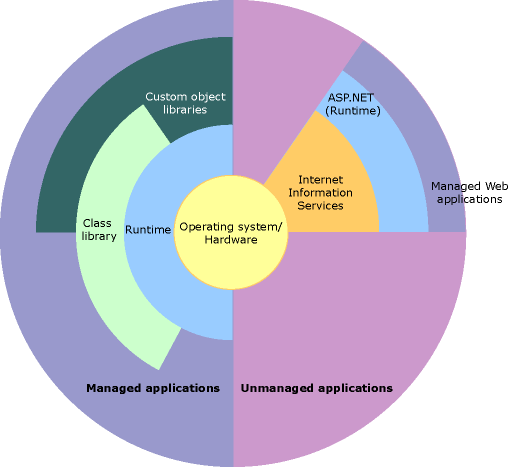
\includegraphics[scale=0.6]{img/dotnet-ecosystem.png}
	\caption{Ekosystem .NETa, źródło: \cite{dotnetoverview}}
	\label{fig:dotnet-ecosystem}
\end{figure}

.NET posiada restrykcyjną infrastrukturę weryfikującą poprawność typów i~kodu zwaną CTS (\emph{Common Type System}). CTS sprawia, że cały zarządzany kod jest samo-opisujący. Różne kompilatory, zarówno te stworzone przez Microsoft, jak i~przez inne firmy mogą generować kod zgodny z~CTS. Dzięki temu dowolny kod zarządzany może konsumować dowolne inne zarządzane typy i~obiekty, jednocześnie surowo dbając o~bezpieczeństwo typów. To daje dużą swobodę programistom, którzy pisząc w~dowolnym zarządzanym (w~sensie kompilowanym do kodu zarządzanego .NETa) języku mogą korzystać z~pełnej standardowej biblioteki klas oraz z~zewnętrznych komponentów napisanych w~innych zarządzanych językach.

Do zarządzanych języków należą m.in.\ C\#, Visual Basic .NET, J\#, C++ (specjalna zarządzana odmiana), czy Iron Python (Python kompilowany do CIL). Jednym z~języków platformy .NET jest C\#. Typowany, imperatywny, przypomina Javę, choć jest nowocześniejszy i~ma więcej możliwości(źródło o C\#). Jest to język w~którym będę pisał .NETowe części mojej biblioteki.

Cała platforma .NET jest (słusznie\cite{dotnetrequirements}) kojarzona z~Windowsem, choć można uruchamiać napisane pod nią programy na innych systemach, jeśli tylko posiada się odpowiednią implementację środowiska uruchomieniowego, bo to ono tłumaczy wspólny kod (CIL) na natywne instrukcje (ponownie, znany z~Javy \emph{just-in-time compilation}). Niestety żadna z~alternatywnych implementacji nie wspiera wszystkich funkcji .NET. Dlatego nie można z~pełną swobodą, np. pisać w~C\# pod Linuxa. Jednak dla wielu programów poziom wsparcia jest wystarczający. Chyba najbardziej znana, nie pochodzą od Microsoftu implementacja -- Mono -- nie posiada kilka aspektów, takich jak WPF, WWF oraz ma ograniczone wersje WCF i~stosu asynchronicznego ASP.NET 4.5\cite{monocompatibility}. Ale za to jest dostępna dla kilku systemów operacyjnych, m.in. na Linuxa, Mac OS czy Solaris\cite{monosupportedplatforms}. Także, w~przeciwieństwie do standardowej maszyny wirtualnej Microsoftu, może działać na architekturach procesorów innych niż x86 i AMD64\cite{dotnetrequirements}, np. na ARM, PowerPC, SPARC.

%\subsection{Odpowiedniość Javy i C\#}
%Porównać zdolności obu języków, znaleźć cechy nieprzetłumaczalne. Jak dużą zgodność można uzyskać teoretycznie?
%
%\url{http://stackoverflow.com/questions/78811/is-there-an-effective-tool-to-convert-c-sharp-code-to-java-code}\\
%\url{http://en.wikipedia.org/wiki/Comparison_of_C_Sharp_and_Java} tu wyjątkowo zacytuję Wikipedię, bo dobry artykuł\\
%\url{http://msdn.microsoft.com/pl-pl/library/ms836794.aspx} porównanie microsoftu
%
%Po prostu jest trochę różnic i nie wszystko się będzie dało przetłumaczyć 1 w 1. Ale i tak wszystkie cechy języka trudno będzie przetłumczyć. Np. propertiesy, adnotacje
%
%\subsection{Python}
%Pierwsza platforma jaką rozważałbym jako alternatywę dla podstawowych (Androida i .NETa) do implementacji mojej biblioteki. A to dlatego, że jest moją ulubioną. I może chodzić praktycznie na wszystkim.
%
%Z drugiej strony, ten projekt może nie mieć dla niego sensu, bo jest duck typing. Nie musi być faktycznych związków między typami. Jeśli jakieś pola albo metody znajdą się w trakcie odpalania, to dany obiekt może być uważany za taki typ. Ale nie ma żadnego problemu z zachowywaniem zależności. Właściwie można wszystko wysłać bez etykiet jako proste JSONy. Nawet jak nie zachowamy nazw typów, to mniej więcej wszystko będzie działać.
%
%Nie platforma a język, ale w sumie chodzi na wszystkim. I na windowsie, linuxie i androidzie. Lubię też w nim pisać. Można go sportować.
%
%Wzmianka, że podstawowa implementacja pythona, której będę używał (albo i nie) nie korzysta z wielu procesorów.

\section{Serializacja (TODO)}
\subsection{Ogólnie}
Serializacja polega na przetworzeniu obiektu (lub grupy obiektów, lub innej struktury danych z~pamięci) w~postać nadającą się do zapisu na dysk albo do transportu przez sieć\cite{serializationbasics}. Nieodzownie łączy się też z~deserializacją -- odwrotnością serializacji, która odtwarza w~pamięci obiekt z~zapisu na dysku lub z~danych z~sieci. Kiedy będę używał określenia serializacja zazwyczaj w~domyśle będę mówił i~o~serializacji, i~o~deserializacji. Podstawową techniką serializacji jest ``spłaszczenie'' obiektu w~jednowymiarowy strumień bitów, a~następnie, w~ramach deserializacji, na odtworzenie z~tego strumienia oryginalnego obiektu.

Warto zaznaczyć, że możliwe jest przeniesienie obiektu z~jednej platformy programistycznej na drugą (przetłumaczenie z~jednego języka programawania na inny) przez jego serializację na platformie źródłowej, a~następnie deserializację na docelowej.

Najczęściej kiedy mówi się o~serializacji nie ma się na myśli, jednak, tworzenia przenośnego (bo to cecha danych zserializowanych) ciągu bajtów. Zazwyczaj chodzi o~tekstowy zapis obiektu, mniej lub bardziej czytelny dla człowieka. Formy binarne wymagają raczej przetworzenia przez program aby sprawdzić poprawność lub ocenić, co reprezentują. W~przypadku reprezentacji tekstowej, człowiek może zidentyfikować zawartość i~poprawność po prostu czytając dokument (można tak nazwać wynik serializacji).

Serializacja binarna (do strumienia bajtów/bitów) jest na ogół szybsza i~daje mniejsze rozmiary dokumentu\footnote{Można nawet uzyskać brak narzutu względem reprezentacji obiektu w~pamięci.} niż serializacja tekstowa.
Ale obiekty przez nią zapisane mogą być trudne do odtworzenia na innych systemach operacyjnych niż źródłowy, z~uwagi na możliwą niezgodność kolejności bajtów (ang.: \emph{endianness}). Wiele platform programistycznych, np. Java i~.NET, posiada zdolność serializacji binarnej, jednak tworzone zapisy nie są zgodne; strumień bajtów przedstawiający obiekt stworzony przez jedną platformę na ogół jest nieczytelny dla drugiej.

Serializacja tekstowa jest dużo popularniejsza od binarnej, przynajmniej w~aplikacjach heterogenicznych i~internetowych. Jest łatwiejsza w~rzeczywistym (np. biznesowym) użyciu, szczególnie podczas korzystania z~języków wysokopoziomowych.
Niestety wiąże się na ogół ze sporym narzutem rozmiaru danych\footnote{Szczególnie jeśli obiekt zawiera surowe dane binarne,np. w~formie tablicy bajtów, czy bitmapy.} i~prędkości ich przetwarzania.
Ale za to można uzyskać prostotę i~przenośność obiektów na różne platformy programistyczne.

Zapis przenośnej formy obiektów nie jest trywialny. Jeden obiekt może być powiązany z~wielką siecią innych. Czasem te połączone obiekty faktycznie zawierają się w~serializowanym, są jego logiczną częścią. Niekiedy można natrafić na duży zbiór zależnych, równoważnych sobie obiektów. W~sieci powiązań mogą też pojawić się cykle, sprawiające problemy dla automatów trawersujących graf (właśnie w~takiej formie można przedstawić obiekt) obiektu.

W~związku z~tymi problemami nie zawsze możliwe jest zachowanie pełni oryginalnych danych w~transporcie.
Ale świadomość ograniczeń serializacji w~projektowaniu swoich obiektów oraz asortyment potężnych narzędzi (o~których będzie mowa w~tej pracy) pozwalają przenieść niemal wszystko.

%Niestety przekazywane obiekty nie mogą mieć żadnej większej logiki związanej z dostępem do swoich danych. O ile można zmapować pola klasy w jednym języku na pola w drugim, to przetłumaczenie metod dostępowych, które mają jakąś logikę (np. zmień licznik odczytań, kiedy czytam zmienną) w automatyczny sposób byłoby niemal niemożliwe (wymagałoby automatu rozumiejącego sens kodu -- programu programisty).

%Binarnie można teoretycznie zapisać obiekt z pamięci jakiegoś języka nie tracąc niby żadnych informacji (chociaż powiązania dalej są problemami).
%Ale to nigdy nie będzie standardowe. Tekstowo też bym mógł w niestandardowy sposób zachować wszystko.

%A Marshalling?
%http://stackoverflow.com/questions/154185/what-is-object-marshalling
%http://stackoverflow.com/questions/770474/what-is-the-difference-between-serialization-and-marshaling
% W sumie to prawie to samo co serializacja, ale wiąże się niejako z przekazem większego sensu. Ma, chyba, na celu odtworzyć obiekt z jego tożsamością, a nie tylko jego kopię.

\subsection{Typy zapisu}
Zarówno serializacja binarna i tekstowa ma wiele odmian, o różnym stopniu rozpowrzechnienia (a więc niejako tworzących standard). Tutaj niektóre zostaną przybliżone.

Powiem tu tylko o tych bardziej standardowych. Np. jak Java sobie serializuje do bajtów mówić nie będę.
W sumie każdy z nich pozwala uzyskać ustrukturalizowane dane.

O każdym kilka zdań - jaka jest ich główna misja:
XML - ustrukturalizowany i w ogóle, chyba najpopularniejszy
JSON - drugi pod względem popularności, czytelniejszy i lżejszy
BSON - binarny, MongoDB
YAML - ma też coś poprawiać, używa go Ansible
AXON - ma być w ogóle super, ale mało popularny jeszcze

Podać przykładowy obiekt w C\# i wypełnienie go danymi. Przedstawić jego reprezentacje w różnych formatach (dla XML może wyglądać różnie, bo mogą być elementy, mogą atrybuty).

Mogą być formaty dopasowane do konretnego programu, języka albo bardziej uniwersalne.
Może być dopasowan do jednego typu danych i jednego zastosowania (se sam napisałem jak moja klasa ma się zapisywać i odtwarzać), a może być bardziej dynamiczna i uniwersalna (binding w WCF albo JAX-WS)

SOAP, tutaj, czy potem?

Jak się oznacza typy (że pole jest jakiejś klasy), np. w JSONie (JsonDataContractSerializer). W SOAPie są domyślnie, wszystko ma typ konkretny i jest bardzo ściśle.

\url{http://bsonspec.org/}\\
\url{http://json.codeplex.com/} -- w sumie to to tylko przykład implementacji dla .NET\\

\url{http://intellimath.bitbucket.org/blog/posts/axon_overcomes_json.html}\\
\url{http://intellimath.bitbucket.org/blog/posts/axon_best_of_json_xml_yaml.html}\\
Jakieś porównanie AXONa i JSONa. Jeśli AXON jest stabilny i wspierany na Androidzie i .NETcie (bardzo ważne) to powinienem go użyć, bo przecież parę problemów rozwiązuje.

Oznaczanie typów, takie jawne, kiedy nie jest to pewne.

Tu coś napisać może o tym, że nie wszystkie cechy obiektu, na jakie pozwala język dają się zapisać tymi metodami. Chociaż, może to bardziej rzeczy związane z klasą są ciężkie do opisu, a jak mamy klasy opisane w normalnych językach a tylko obiekty zapisujemy, to może być spoko.

\subsection{Binding}
\url{http://rpbourret.com/xml/XMLDataBinding.htm}\\
Pomagają przy automatycznej serializacji.



A może najlepszym rozwiązaniem będzie generator customizowalnych bindingów (może nawet do JSONa) z wygodną konfiguracj)? Raz by się generowało mapowanie i wszystko działa na zawsze. 

Czasem trzeba pomóc z palca, coś napisać, nadać etykietki, z czegoś zrezygnować. Czasem może działać automat. Zależy, jak zaprojektowane są dane, z jakiego języka pochodzą i jakich narzędzi używamy.

NA TYM BĘDZIE DZIAŁAŁO TŁUMACZENIE KLAS
W WSDL poza opisami operacji realizowanych przez usługę znajdują się też pliki XSD opisujące wszystkie struktury danych (klasy), które będą wymieniane. Dla tego posiadając WSDL usługi możemy wygenerować wszystkie klasy potrzebne do stworzenia klienta usługi.

Złożony problem pojawia się wtedy, kiedy servicy mają działać w obie strony wykorzystując te same klasy danych. W bardziej skomplikowanych systemach rozproszonych może się pojawiać taka sytuacja. Załóżmy istnienie dwóch aplikacji: A i B. Są one napisane w różnych językach. Każda z nich udostępnia usługę zwracającą obiekt danych X. A korzysta z usługi wystawianej przez B, a B korzysta z usługi wystawianej przez A. Mimo tego, że obiekt X w obu aplikacjach będzie zawierał te same dane, to jednak jego kod będzie inny. Dlatego nie można mówić o jednej klasie X, a o dwóch. Nazwijmy je XA i XB. TUTAJ DALEJ WYTŁUMACZENIE PRZYKŁADU AŻ W KOŃCU DOJDZIEMY DO TEGO, ŻE TRZEBA NAPISAĆ KLASĘ W JEDNYM JĘZYKU, POTEM ZROBIĆ JEJ BINDING DO XSD I Z XSD DO DRUGIEGO JĘZYKA.

Problem przesyłania typów polimorficznych (coś przeczytać, może). Ogólnie raczej się opisuje co ma być powiązane w jakiś modelach.

Ciężko o pełną swobodę w korzystaniu z obiektowości używanych przeze mnie języków, czyli Javy i C\#. Oba niby są obiektowe, ale przy przechodzeniu przez warstwę zdalną potrafią tracić tę właściwość

Może być różnie sparametryzowana i dawać rózne postaci dla takich samych obiektów, zależnie od tego, jak powiążemy xmla z klasą.\\
\url{http://www.codeproject.com/Articles/483055/XML-Serialization-and-Deserialization-Part} w XML Serialization and Attributes\\

\url{http://json-schema.org/}\\

\subsection{SOAP}
Wykorzystywny przy dużych web serviceach. Forma XMLa. Opisuje obficie całe wołanie i wykorzystywane dane.

\section{Zdalne wywoływanie kodu(TODO)}
Tu rozstaną opisane techniki umożliwiające zdalne wywoływanie kodu.

Zrób tak, żeby najpierw zarysować RPC, web servicy itp a dopiero potem wiązanie danych (żeby było wiadomo po co jest)

Dane (argumenty metod i~wartości przez nie zwracane) wymieniane pomiędzy klientem a serwerem będą miały postać obiektów (programowanie obiektowe). To znaczy, że typy dziedziczące i implementujące ten sam interfejs będą polimorficzne (źródło!). Często normalnie nie jest tak łatwo to osiągnąć w heterogenicznych środowiskach - ciężko o zachowanie związków między klasami po mapowaniu na drugi język

Ogólnie trochę o RPC. Że wiele technologii to RPC (Web service'y, CORBA), że to zawiera i tłumaczenie i transport.
Wywoływaniu kodu w innym procesie lub na innym kompie.

\url{http://stackoverflow.com/questions/12450404/json-pojo-consumer-of-polymorphic-objects}

Web-servicey, XML-RPC, REST z JSONem i XMLem. 

\subsection{Transport danych}
Potrzebny, żeby coś wywołać. Bo trzeba przetransportować chociażby oznaczenie, jaką metodę chcemy uruchomić. Można też przekazać parametry, oraz zwrócić wartość z~powrotem.

Też bardzo szeroka dziedzina. Jak już się przetłumaczy, to zawsze trzeba jakoś przetransportować. Jak możemy przekazywać w ramach jednego kompa, jak pomiędzy kompami lokalnie, jak globalnie.
Celuję w globalnie, ale zwsze szerszą metodę można zastosować wężej (chociaż może nie być tak wydajna jak te węższe)

JAKIŚ OBRAZEK Z WARSTWAMI KOMUNIKACYJNYMI - FIZYCZNA, PAKIETY, TCP/IP, HTTP, SSL

Nie będę się więcej na tym skupiał, to zagadnienie dla telekomunikacji. Ogólnie ta tematyka będzie u mnie w pracy pomijana i będę korzystał tylko z gotowych klocków (warstw) bez głębszego zastanowienia nad nimi. 

\emph{TEŻ PRZYDAŁBY SIĘ JAKIŚ ARTYKUŁ CHOCIAŻ}

\emph{TCP, PIPEy, SSL, HTTP, HTTPS}

\subsection{XML RPC}
Podstawowy chyba obecnie przykład RPC. Proste to.
\url{http://xmlrpc.scripting.com/default.html}\\
\url{http://xmlrpc.scripting.com/spec.html}\\
\url{http://effbot.org/zone/xmlrpc-errata.htm}\\

\subsection{Usługi internetowe (\emph{web services})}
W sumie to przykład tłumaczenia danych  i transpotru.

SOAP ma faulty -- ważną rzecz w obiektowych językach (exception).

Jeden ze sposobów na zdalne wywoływanie kodu to usługi internetowe. Korzystając z otwartych standardów takich jak XML, SOAP, WSDL i UDDI umożliwiają integrację aplikacji poprzez Internet. XML jest używany do etykietowania danych, SOAP do ich pakowania i transferu (alternatywnie można używać też RESTa lub JSONa), WSDL opisuje interfejs usługi, a UDDI dostarcza spisu dostępnych usług (on nie leży w naszym obszarze zainteresowań). SOAP i WSDL są zapisywane przy pomocy XML. Web servicy używane są najczęściej do komunikacji aplikacji komercyjnych (np. serwery, portale) ze sobą lub z klientami. Pozwalają organizacjom na wymianę danych nie wymagając wiedzy o wewnętrznej strukturze informatycznej za firewallem.

W przeciwieństwie do tradycyjnych modeli przetwarzania typu klient – serwer, takich jak np. system stron internetowych, usługi internetowe nie mają graficznego interfejsu użytkownika. Służą one do dzielenia logiki biznesowej, danych i procesów poprzez sieć, przy pomocy jednolitego interfejsu programistycznego. To aplikacje się komunikują, nie użytkownicy. Programiści mogą, co prawda, dodać usługę internetową do aplikacji, która posiada GUI (np. aplikacja okienkowa lub strona internetowa) aby zaoferować zwykłym użytkownikom jej funkcjonalność.

Usługi internetowe pozwalają różnym aplikacjom wykonanych w różnych technologiach (np. całkowicie odmienne języki programowania) na porozumiewanie się ze sobą bez potrzeby czasochłonnego tworzenia kodu tłumaczącego. Nie ma też znaczenia to, czy obie aplikacje znajdują się na jednej maszynie, czy po drugiej stronie świata.
Usługi sieciowe na platformie .NET realizowane są w ramach WCF. Javie obecnym standardem jest JAX-WS.

co to webservicy i po co są?\\
do czego mogą się przydać na androidzie?\\
dlaczego ich nie ma? Chyba stwierdzili, że ogólne web servicey są za ciężkie i za bardzo obciążają (Windows phone też nie ma WCF)\\

Druga rzecz, którą chcę uzyskać to możliwość łatwego tworzenia programów współpracujących między wyżej wymienionymi platformami. Kiedy wywołujemy zdalny kod często trzeba przekazać mu jakieś parametry, często też chcemy otrzymać wartości zwrotne. Pomijając sam fakt transportu danych z jednej platformy na drugą stajemy przed problemem niezgodności typów danych. Wiemy, że na obu końcach będą użyte dwa różne języki, więc struktury danych nie będą kompatybilne. Trzeba temu zaradzić.
Ogólnie ujęte rozwiązanie dla powyższych problemów to serwer usług internetowych (ang. web services) wraz z narzędziami. Dzięki mechanizmowi usług sieciowych można wykonać dowolny kod na serwerze nie zależnie od technologii wykorzystywanych po obu stronach. Nie istnieje jeszcze (przynajmniej nie udało się znaleźć) serwer web service’ów dla Androida. Istnieją za to biblioteki pozwalające na przetłumaczenie klas z C\# na Javę.

WCF to webservice'y, a jednocześnie rekomendcja microsoftu na komunikację między procesami (co prawda na innym bindingu), tak że web servicey są dość uniwersalne i dobre nie tylko w dużej sieci do komunikacji między aplikacjami.

WSDL -- tylko on zapewnia używalność (cytat z RESTful).

\subsection{REST}
Cośtam o RESTcie \url{http://www.oracle.com/technetwork/articles/javase/index-137171.html}\\
REST and POX \url{http://msdn.microsoft.com/en-us/library/vstudio/aa395208(v=vs.90).aspx}\\

Korzysta z XMLa lub JSONa, ale raczej nie z SOAPa.

Restful web services vs ``big'' web services: \url{http://www2008.org/papers/pdf/p805-pautassoA.pdf}\\
\url{http://www.infoq.com/articles/rest-soap-when-to-use-each}\\

WADL -- taki WSDL. Ale rzadko używany raczej. Cytat z restful web services.

Błędy można zwracać wiadomościami HTTP, ale jak z ich obiektowym odczytywaniem?